\documentclass[conference]{IEEEtran}
\IEEEoverridecommandlockouts
% The preceding line is only needed to identify funding in the first footnote. If that is unneeded, please comment it out.
\usepackage{cite}
\usepackage{xurl}
\usepackage{amsmath,amssymb,amsfonts}
\usepackage{algorithmic}
\usepackage{graphicx}
\usepackage{textcomp}
\usepackage{xcolor}
\usepackage{cleveref, array, booktabs, threeparttable}
\usepackage{kotex}
\usepackage{makecell}
\usepackage{float}
\usepackage{subcaption}
\usepackage{tabularx}
\usepackage{longtable}
\usepackage{multicol}
\usepackage{listings}
\usepackage{cleveref, array, booktabs, threeparttable}
\usepackage{tabu} 
\usepackage{enumitem}
\usepackage[export]{adjustbox}
\def\BibTeX{{\rm B\kern-.05em{\sc i\kern-.025em b}\kern-.08em
    T\kern-.1667em\lower.7ex\hbox{E}\kern-.125emX}}

\begin{document}

\title{DANBI – My Home’s Water Secretary\\
{\footnotesize \textsuperscript{*}Team Name : LeGend}

}

\author{\IEEEauthorblockN{Kim Eunho}
\IEEEauthorblockA{\textit{dept. Information System} \\
\textit{Hanyang Univ.}\\
Seoul, Republic of Korea \\
applejam5@naver.com}
\and
\IEEEauthorblockN{Oh Jiyun}
\IEEEauthorblockA{\textit{dept. Information System} \\
\textit{Hanyang Univ.}\\
Seoul, Republic of Korea \\
baram0516@naver.com}
\and
\IEEEauthorblockN{Jeong Hyoeun}
\IEEEauthorblockA{\textit{dept. Information System} \\
\textit{Hanyang Univ.}\\
Seoul, Republic of Korea \\
gydms415@hanyang.ac.kr}
\and
\IEEEauthorblockN{Choi Soojung}
\IEEEauthorblockA{\textit{dept. Information System} \\
\textit{Hanyang Univ.}\\
Seoul, Republic of Korea \\
tnwjd5127@naver.com}

}

\maketitle

\begin{abstract}
Now that humans, pets, and plants all live in a family, there are many things to care about and it is becoming difficult to manage them at once. We developed 'DANBI' that intuitively manages water intake information of all members of our family at once focusing on water, which is the basis of all life. DANBI is our water secretary which informs us when necessary with convenience through technical linkage with LG PuriCare water purifiers and NUGU speakers.
\end{abstract}

\begin{IEEEkeywords}
water secretary for family, water intake managing application, LG PuriCare water purifier, NUGU, and etc.
\end{IEEEkeywords}

\ 

\begin{table}[ht!] \renewcommand\arraystretch{1.25}
  \begin{threeparttable}
      \caption{Role Assignments%
      \label{tab:table1}}    %% Caption above tabular, label inside caption
      \begin{tabular}{@{}l l>{\raggedright\arraybackslash}p{3.8cm}@{}}
      \toprule
      \bfseries Role & \bfseries Name & \multicolumn{1}{l}{\bfseries Task description and etc.} \\
      \midrule
      User & Oh Jiyun & Think of ideas and design functions to improve usability. Specify people's need and suggest how to implement it as service functions. \\
      Customer & Jeong Hyoeun & Examine the service of the competitors and plan functions that could be our differentiator from others. Consider UI design which can attract the customers. \\
      Software developer & Choi Soojung & Be responsible for software development. Understanding user needs, developing software solutions, monitoring performance and modifying programs as needed. \\
      Development manager & Kim Eunho & Make a plan in order and quarterly to achieve the project's goals. Assign team members to their own roles and continuously check the progress of the work. \\
      \bottomrule
      \end{tabular}
  \end{threeparttable}
\end{table}

\ 

\section{Introduction}

\subsection{Motivation}\label{AA}
\setlength{\parindent}{2ex}
Water is the most fundamental factor in maintaining a person's life. Drinking insufficient water increases the risk of exposure to various diseases such as kidney stones, obesity, diabetes, bladder cancer, and colon cancer. Nevertheless, the proportion of 'people who intake sufficient water' decreases every year, and 6 out of 10 people are reported not to have enough water. Therefore, there is a need for a service that properly helps with water intake, and we developed this service using applications and AI speakers.

At the same time, this service allows you to manage the water supply of pets and plants together. In modern society, the form of family is changing. More and more people live with pets and plants, and unlike before, they begin to regard them as family members. As a result, people became more interested in their health care. For pets and plants, water intake is directly related to maintenance of life. In the case of pets, insufficient water intake can lead to diseases. Typically, it damages the kidneys and pancreas, which leads to renal failure and pancreatitis. For plant, water is a carrier of nutrients, which extracts nutrients from the soil and transports them to the end of the plant's leaves. Without enough water in cells, plants become malnourished and unable to support their own weight. Therefore, we created DANBI that helps manage water intake of humans, pets, and plants, that is, all of our family.

DANBI is a pure Korean word that means rain that falls appropriately when necessary. Like rain that falls when necessary on dry land, it means that it helps humans, pets, and plants drink proper water through notifications in busy modern society.

\ 
\subsection{Problem Statement}
\setlength{\parindent}{2ex}
People fully understand that all creatures have to take water enough. However, do you know how much water do you drink daily? Probably, most of people would not be able to figure out the amount of water they intake. Besides, the interval of drinking water is also important as the quantity of water people drink. But drinking water regularly is not easy for busy modern people. This is same for taking care of water intake of pets and plants which are part of our life. Therefore, the function which records water intake of people, pets and plants at our home, and sends notifications periodically will be a great help for us. Of course, there are several mobile applications providing service like this, but they have some inconvenient problems.

To use mobile applications which manage water intake of people or pets, the users have to write the amount of water they drink in person everyday. This way is very annoying since the users have difficulty to know exact quantity of water they intake. However, DANBI provides recommended water intake based on the user's physiological information. If the users respond to pop-up notification or voice guidance from NUGU speaker, the recommended intake(or user setting of the amount) will be recorded automatically. DANBI also works with LG PuriCare Water Purifier, so that the amount of water from LG PuriCare Water Purifier will be uploaded, too.

Nowadays, mobile applications managing water intake overflow in the market, but they are separated for human, for pets and for plants. People who raise pets and plants at their home would be awkward because of this dispersion. A number of mobile applications would make the display messy, and people would be busy recording water intake, moving from here to there. DANBI manages all of these information at once. You can identify the status of water intake related to all of our family member who need water at a glance with only one mobile application.

You can use DANBI easier with AI speaker NUGU. DANBI sends notification of water intake by not only mobile application, but also speaker voice using NUGU speaker. Also, users can respond to speaker with voice, and record will be uploaded as the response to pop-up notification.

Additionally, DANBI is linked to LG PuriCare Water Purifier, so that it can manage water intake efficiently. When you select '물 받기' option to the notification, LG PuriCare Water Purifier will provide the amount of water drunk at once. Some people prefer cold water, and others prefer warm water. LG PuriCare Water Purifier provide appropriate temperature of the water based on the users' preference set in DANBI. Users can intake water easily with the temperature they want.

\ 
\subsection{Research on Related Software}
You can find applications in the App Store and Play Store (Apple and Android) that manage water intake of humans, pets, and plants.\\
\begin{enumerate}
\setlength{\parindent}{2ex}
\setlength{\parskip}{0.5em}
\item 나의 물 

First of all, there is an app, named '나의 물', that manages human water intake. It ranks 28th in the charts of the health and fitness sectors.(Apple App Store, as of October 11, 2021) When a user enters weight and height, the standard amount of daily water intake is provided. And a notification is sent at a set notification interval calculated from input wake-up time and bedtime. It also helps to record my water intake information. In addition to water, you can record drinks such as coffee, tea, carbonated water, and juice, and the rest of the drinks except water are recorded by calculating the ratio. You can get visualized results of how much you have reached water intake goal in a day, a week, or a month and share it with your registered friends. You can also check the association between water intake and weight change by recording weight changes.
\item 물 알림 - water reminder 

Another app that manages human water intake is '물 알림 - water reminder'. Like the app introduced earlier, when a user enters weight and height, it calculates the daily water intake standard and sends notifications according to the set notification time. In addition, you can record your water intake information on the app and provide not only water but also various beverage information such as coffee and beverages. It is noteworthy that recording the type and intake of beverages consumed automatically calculates and provides nutritional information such as calories, protein, fat, carbohydrates, caffeine, and sugar. The water intake goal is calculated according to gender, age, weight, height, and activity level. The arrival information on the water intake goal is shown weekly and monthly on a graph, but there is no function to share it with others. If the goal is reached continuously for a specific period of time, the award details are stamped to raise awareness of the goal.
\item 집사일기

An app that manages pet water intake and comprehensive health is '집사일기'. The app provides basic intake health information such as recommended drinking amount and feed intake depending on the weight of the pet. Through this app, you can enter health-related data such as weight of your pet, feed, drink amount, heart rate, and animal heat. In addition, a list of abnormal symptoms is provided so that if there is some problem in the health of the pet, it can be checked quickly. It helps comprehensive health care for pets by allowing you to manually enter hospital test results or take pictures of test tables to register.
\item Into Pet 

'IntoPet' is an app that helps you manage your pet's health. Through the hospital notebook function, you can manage your pet's visit, vaccine history, medication, and expected date of your next visit. You can take care of your pet's walk, diet, and drinking through the health notebook function. In the diet management function, feed, snacks, and drinks are recorded and used as basic information for health care. However, it does not provide the recommended intake and is an app that functions as a hospital notebook rather than a health notebook.
\item Plantgram 

There is a 'Plantgram' application that helps to check the plant water cycle. If you select the provided plant species, then application automatically sets the cycle of watering, nutritional supplements, and repotting. If you record the last watering day, it sends a notification so that you won't forget the watering day according to the cycle. You can also see other people's plants or get information through the community. It also provides AI plant recommendation according to your lifestyle.
\end{enumerate}
There are many applications that provide such useful functions, but information on humans, pets, and plants cannot be managed at once, and in person input should be accompanied for each water intake. All of your family water intake information should be checked through different applications, and notifications should be received from each application. People would feel a great inconvenience in the distribution of this information, so we suggest a solution called DANBI.

\ 
\ 

\section{Requirements}

\begin{itemize}
\setlength{\parindent}{2ex}
\setlength{\parskip}{0.5em}
\item \textit{Sign Up}

A user can download and click DANBI application in the App Store or Google Play Store. Then, the entry page will appear for a while and the user enters the login page. The user can sign up and log in on the login page, but if she is not a member, she must sign up. If the user clicks the sign up button at the bottom of the login page, she will go to the sign up page. Sign up is possible in two main ways. There are through general sign up and social sign up. General sign up is made by entering non-overlapping e-mails, passwords, names, and mobile phone numbers. Mobile phone numbers are used to reset passwords. Social sign up is also possible with social ID of Google, Naver, and Kakao without a separate authentication procedure.
\item \textit{Login}

The user can log in when she completes her sign up procedure. Login is also possible with general login and social login. By entering an email and password, the software checks whether the information is in the database, and if the information is present, the user can succeed in logging in. If the user tries to log in with wrong information that does not exist in the database, she will receive a message saying, "Your ID or password is incorrectly entered." There are ID search and password reset buttons under the login button. If the user presses the button, she can find her ID and reset password through personal information. The user who succeeds in logging in can access the main page.
\item \textit{Member registration}

If the user succeeds in logging in, she will go to the main page. On the main page, after pressing the + button, each physiological information may be input to add a family member. Family member’s information can be registered through DANBI application. The physiological information to be registered by each individual is as follows.  
\begin{itemize}
    \item Human: Nickname, Weight, Wake-up/bedtime, Preferred water temperature, Water intake goal, and Water intake cycle.  
    \item Pet: Nickname, Animal type (dog/cat), Weight, Wake-up/bedtime, Water supply goal, Water supply cycle   
    \item Plant: Nickname, Plant type, The last water supply date, The water supply time, Water supply at once, Water supply cycle. 
\end{itemize}

If the user presses the name of each member, she will go to the page where each physiological information is presented. If she presses the modify button on each page, she can modify the set physiological information.
\item \textit{Recommended daily water intake}

The recommended daily water intake is automatically provided by the server based on the physiological information entered into DANBI application. The provided amount appears in the application, and the user can check it through the screen of the application. Statistical recommended water intake is provided, but it can be set and changed directly according to the user's taste. This soon becomes the user's water intake goal. Once all physiological information and water intake goal have been set, the setting is completed by pressing the registration button. DANBI application provides recommended daily water intake to humans, recommended daily water supply to pets, and water supply at once to plants. 
\item \textit{Water intake cycle}

It provides humans with a recommended water intake cycle. Pets are provided with a recommended water supply cycle. Plants are provided with recommended water supply cycle according to species. This is provided by the server based on statistics, but can be changed and set as desired by the user.
\item \textit{Calculate water intake at once}

After setting the water intake goal, water intake at once is calculated by daily water intake goal and water intake cycle. In the case of humans, water intake at once is calculated through a series of processes, and the process is as follows.
\begin{enumerate}
\setlength{\parindent}{2ex}
\item Calculate the time spent awake from bed and wake-up time entered when registering physiological information.

\item Provide a recommended water intake cycle for human, and calculate the number of times the user drinks water a day based on the time she is awake and the daily water intake goal.

\item Calculate the water intake at once by dividing the daily water intake by the number of times she drinks water.
\end{enumerate}

The same is for pets, but instead of water intake, words are replaced with water supply to calculate and provide water supply at once.  In the case of plants, since water supply at once varies for each size, it is assumed that the user directly sets it.
\item \textit{Calculate the next water supply date for plants}

The next water supply date is calculated by the last water supply date and water supply cycle input when registering physiological information. This can also be directly changed and set by the user.
\item \textit{Notification}

When it is time to water intake, the user can receive a notification. The notification is possible by both DANBI application and the NUGU speaker.

In the case of an application, there are two main types: a pop-up notification and a push notification. A pop-up notification appears when the user is using a mobile phone, and a push notification appears when not using it. When the water intake time comes, the user's name and the amount of water intake at once are shown as pop-up notifications or push notifications. There are three option buttons below this notification. The user can select one of the three reaction option buttons, and when selected, the user requests a reaction to the server.

NUGU speaker also provides notification of water intake time. When the water intake time comes, the user's name and the water intake at once are notified by voice. The user can respond to the notification in three ways, which causes the server to request work on the response.
\item \textit{User Response}

User can select the response that they want to the notification from application or NUGU speaker by choosing the application option or answering NUGU speaker. Both application and NUGU speaker provide same options, and perform same tasks. These are the options that user can choose.
\begin{enumerate}
\setlength{\parindent}{2ex}
\item 물받기

The option '물받기' is the feature which gets water from LG PuriCare Purifier and updates user's water intake information.

When the user selects the option '물받기' at the application's notification, DANBI requests tasks about the option '물받기' to the server. Server sends a query to LG PuriCare Purifier asking water from it. The query contains user's water intake per serving and preferred water temperature. LG PuriCare Purifier receives the query and supplies water set to user information. Server updates that user took in water per serving with the current time information.

User can also select this option to NUGU Speaker. When the user says "물 받아줘" to NUGU Speaker's notification, NUGU Speaker requests tasks about the option '물받기' to the server. Server sends a query to LG PuriCare Purifier asking water from it. The query contains user's water intake per serving and preferred water temperature. LG PuriCare Purifier receives the query and supplies water set to user information. Server updates that user took in water per serving with the current time information.
\item 마시기

The option '마시기' is the feature which updates the information that user drank water per serving voluntariliy. The difference from '물받기' is that user voluntarily takes water, not from LG PuriCare Purifier. This option is useful when user intakes drinks except for water from purifier(eg. water bought from outside, tea).

When the user selects the option '마시기' at the application's notification, DANBI requests tasks about the option '마시기' to the server. Server updates that user took in water per serving with the current time information.

User can also select this option to NUGU Speaker. When the user says "물 마실게" to NUGU Speaker's notification, NUGU Speaker requests tasks about the option '마시기' to the server. Server updates that user took in water per serving with the current time information.
\item 미루기

The option '미루기' is the feature which user chooses when the user can't drink water immediately. If user can't intake water at the time they receive notification, user can prevent automatic update by selecting the option '미루기'.

When the user selects the option '미루기' at the application's notification, DANBI transfers the option '미루기' to the server. Server doesn't update water intake information.

User can also select this option to NUGU Speaker. When the user says "나중에 마실게" to NUGU Speaker's notification, NUGU Speaker transfers the option '미루기' to the server. Server doesn't update water intake information.
\end{enumerate}

\item \textit{Checking the amount of water intake} 

User can check the amount of water intake of all family members. When user selects the certain member from 'main page', DANBI shows today's water intake status by graph. This graph shows the proportion of the current amount of water to water intake goal based on records stored in the server.

User can also check the amount of water intake of family members. When user asks certain member's daily amount of water intake to NUGU Speaker, NUGU Speaker requests information about today's water intake and water intake goal to the server. NUGU Speaker provides the amount of water intake up to now and the rest part of water intake goal by voice.
\item \textit{Checking the date/time of water intake} 

User can check the time of water intake of all family members. When user selects the certain member from 'main page', DANBI shows records of water intake. In case of humans and pets, who have to drink several times in a day, DANBI shows today's water intake records. In case of plants, which has long cycle of water intake, DANBI shows its most recent water supply record. Also, DANBI indicates family member's next planned water intake time at the bottom.

User can also check the last time and next time of water intake of all family members by NUGU Speaker. When user asks the last time of water intake of the certain family member to NUGU Speaker, NUGU Speaker requests its most recent water intake record to the server. NUGU Speaker provides the most recent water intake record by voice.

When user asks the next time of water intake of the certain family member to NUGU Speaker, NUGU Speaker requests its next planned water intake time to the server. NUGU Speaker provides the next water intake time by voice.
\item \textit{Award stamps}

DANBI provides Awards stamps. User can select the certain family member from 'main page' and check award stamps. In case of humans and pets, they can get a stamp when they achieved water intake goal. In case of plants, they can get a stamp when they got water supply. This is fulfilling for users and encourages steady water intake.
\end{itemize}

\ 

\section{Development Environment}

\subsection{Software Development Platforms}\label{AA}
\setlength{\parindent}{2ex}
\begin{enumerate}
\setlength{\parindent}{2ex}
\setlength{\parskip}{0.5em}
\item React Native
\par \begin{figure}[h!]

\includegraphics[width=3cm]{image/React Native.jpg}
\centering
\end{figure}

React Native is  a JavaScript framework used to develop mobile application for iOS and Android, Web and UWP. It is an open source mobile application framework developed by Facebook. It allows developers to use React along with native platform functions.

\item Node.js
\par \begin{figure}[h!]

\includegraphics[width=3cm]{image/Node.js.png}
\centering
\end{figure}

Node.js is is an open-source, cross-platform, back-end JavaScript runtime environment that runs on the V8 engine and executes JavaScript code outside a web browser. Node.js lets developers use JavaScript to write command line tools and for server-side scripting—running scripts server-side to produce dynamic web page content before the page is sent to the user's web browser. Because it is based on JavaScript, it is easy for front-end developers to understand the code and can lower communication costs. There is an advantage that various functions have been implemented as modules by other developers through npm.

\item Mongo DB
\par \begin{figure}[h!]

\includegraphics[width=3cm]{image/MongoDB.png}
\centering
\end{figure}

MongoDB is a source-available cross-platform document-oriented database program. Classified as a NoSQL database program, MongoDB uses JSONlike documents with optional schemas. We chose MongoDB for our database management because we need free data model not limited in schema.

\item AWS
\par \begin{figure}[h!]

\includegraphics[width=3cm]{image/AWS.png}
\centering
\end{figure}

AWS provides online services for client-side application or other websites. Most services are not exposed directly to end users, but instead offer functionality through APIs for developers to use in their applications. The reason that we chose AWS for backend server is that it is widely used so that we can refer to lots of data. Also, it provides resources for students at reasonable price.

\item Visual studio code
\par \begin{figure}[h!]

\includegraphics[width=3cm]{image/Visual studio code.jpeg}
\centering
\end{figure}

Visual studio code is a source code editor developed by Microsoft for Microsoft Windows, macOS, and Linux. It includes debugging support, Git control, and syntax emphasis functions. It is driven based on Electron framework developed by GitHub.

\item Git/GitHub
\par \begin{figure}[h!]

\includegraphics[width=3cm]{image/Git.jpg}

\includegraphics[width=3cm]{image/GitHub.png}
\centering
\end{figure}

Git is a distributed version management system for tracking changes in computer files and coordinating operations of those files among multiple users. And GitHub is a web service that supports GitStorage hosting, a distributed version management tool. We use version control, back-up, collaboration functions through Git and GiHub.

\item NUGU playbuilder
\par \begin{figure}[h!]

\includegraphics[width=3cm]{image/NUGU playbuilder.png}
\centering
\end{figure}

NUGU playbuilder is a development tool which create NUGU play that understand users' speak and perform appropriate tasks. It is applied to NUGU Speaker, SK Telecom's Artificial Intelligence Speaker. The reason why we chose NUGU playbuilder is to encourage users to use DANBI easily by having conversaton with Artificial Intelligence Speaker. NUGU playbuilder is necessary to run NUGU Speaker.

\item Notion
\par \begin{figure}[h!]

\includegraphics[width=3cm]{image/Notion.JPG}
\centering
\end{figure}

Notion is a comprehensive tool which supports notes, docs, and project management. We made it easy to proceed with the entire project by using the document organization function and collaboration function of Notion. In addition to recording all the conference processes, we also wrote our own ideas, document organization, schedule organization, and reference organization. Each content was organized in separate pages, and the markdown format helped organize documents more neatly.

\item Adobe XD
\par \begin{figure}[h!]

\includegraphics[width=3cm]{image/Adobe XD.png}
\centering
\end{figure}

Adobe XD is a powerful design solution that helps design UI/UX of applications. We used this to design pages and create a prototype of our mobile application, DANBI. Through the various templates in Adobe XD, we were able to design a UI that looks good and is convenient to use. In the process of creating the prototype, we used supported cooperation and sharing functions. By using Adobe XD, we were able to prevent confusion caused by page planning, and save time used to develop.

\item Overleaf
\par \begin{figure}[h!]

\includegraphics[width=3cm]{image/Overleaf.png}
\centering
\end{figure}

Overleaf is an online LaTeX editor. It does not require installation and provides various templates, so you can conveniently work on documents. Overleaf is characterized by being very fast, easy to share, and easy to find errors. In addition, writing in code is convenient to work on because it shows the results on the screen on the right in real time.

\end{enumerate}
\subsection{Programming Language}
\setlength{\parindent}{2ex}

\begin{enumerate}
\item JavaScript
\par \begin{figure}[h!]

\includegraphics[width=3cm]{image/JavaScript.png}
\centering
\end{figure}
JavaScript is high-level, often just-in-time compiled and multi-paradigm. It has dynamic typing, prototype-based object-orientation and first-class functions. JavaScript has several advantages, including speed, simplicity, popularity, interoperability, server load, and rich interfaces. DANBI decided to use React Native as a hybrid web app, and because Node.js is also based on JavaScript, JavaScript is familiar to us and even economical.
\end{enumerate}

\ 

\section{Specification}

\subsection{Mobile Application}\label{AA}
\begin{itemize}
\setlength{\parindent}{2ex}
\setlength{\parskip}{0.5em}
\item \textbf{Entry page}

\par \begin{figure}[h!]
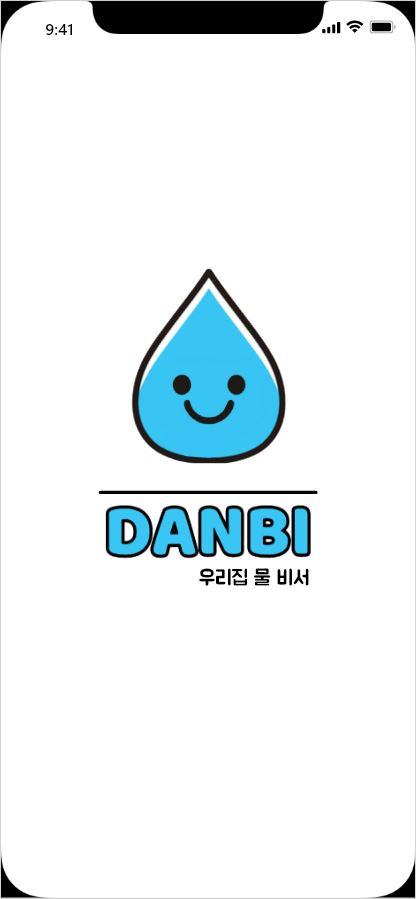
\includegraphics[width=3cm]{xd/entry page.JPG}
\centering
\caption{}
\label{fig:entry}
\end{figure}

[Fig. \ref{fig:entry}] When a user accesses the application, the 'Entry page' will be viewed first. There will be a large droplet icon on the page so that the user can understand the characteristics of application at once. The screen is maintained for 1 second and then automatically connected to the next page. If there is no logged-in account, the application provide a 'Login page'. If user is logged in, the application provide a 'Main page'.

\item \textbf{Sign Up page}

\par \begin{figure}[h!]
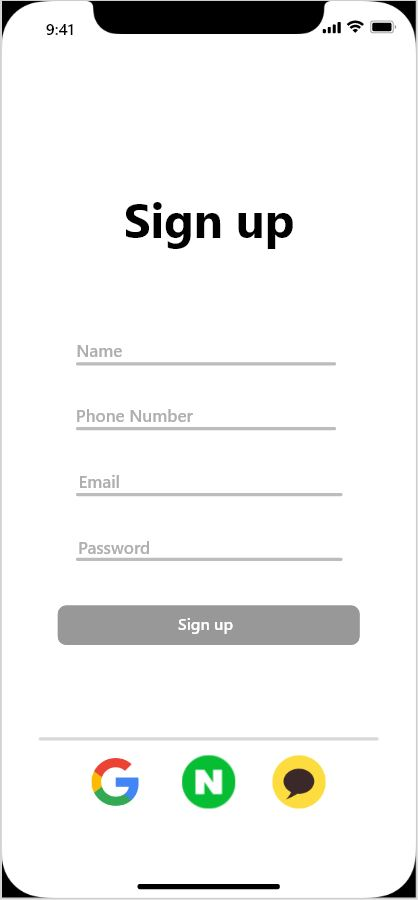
\includegraphics[width=3cm]{xd/sign up page.JPG}
\centering
\caption{}
\label{fig:signup}
\end{figure}

[Fig. \ref{fig:signup}] At the bottom of the 'Login page', user can access the 'Sign Up page' through the sign-up button and can register to DANBI. DANBI provides a general membership function and a membership function through social accounts. The user's information required in the membership registration includes a name, mobile phone number, Email address, and Password.
\begin{enumerate}
\setlength{\parindent}{2ex}
\item Social Sign Up

Social accounts available include 'Google', 'NAVER', and 'Kakao'. When using the social login function, the account is registered with the social ID and Password without a separate authentication procedure. The user's name, mobile phone number, and Email information must be received from a social account, and the user's consent is necessary. When the user presses the agree button, personal information is stored in the DANBI database and the account is created. If the account is successfully created, the user automatically moves back to the 'Login page'.
\item General Sign Up

User can sign up in person by entering 'name', 'mobile phone number', 'Email address', and 'Password'.
\begin{itemize}
\item Name : The name must be text. If the user presses the sign up button without entering or entering a non-text value in the name field, the error message "올바른 이름을 입력하세요." appears as pop-up in the field.

\item Mobile phone number : Mobile phone number must be a number. If the user presses the sign up button without entering or entering a non-numerical value in the mobile phone number field, the error message "올바른 핸드폰 번호를 입력하세요." appears as pop-up in the field. If the user enters the mobile phone number that has already been used for account, the error message "이미 등록된 핸드폰 번호입니다." appears pop up on the field.

\item Email address : Email address must be in the form of an Email. If the user presses the sign up button without entering or entering a value that is not in the form of an Email in the field, the error message "올바른 이메일 주소를 입력하세요." appears as pop up in the field. If the user enters the email address that has already been used for account, the error message "이미 등록된 이메일 주소입니다." appears pop up on the field.
\item Password : Password must satisfy 6-10 digits by combining letters and numbers. If you press the sign up button without entering or entering a Password that doesn't satisfy the conditions in the password field, the error message "올바른 비밀번호를 입력하세요." appears as pop-up in the field. The same process is repeated in the Password verification field. If different values are entered in the Password field and Password verification field, the error message appears pop up in the Password verification field.
\end{itemize}
After entering all input values without errors and pressing the sign up button, 'name', 'ID', 'mobile phone number', 'Email address', 'Password' information is stored in the DANBI database and a new account is created. The application automatically provide the 'Login page'.
\end{enumerate}

\item \textbf{Login Page}

\par \begin{figure}[h!]
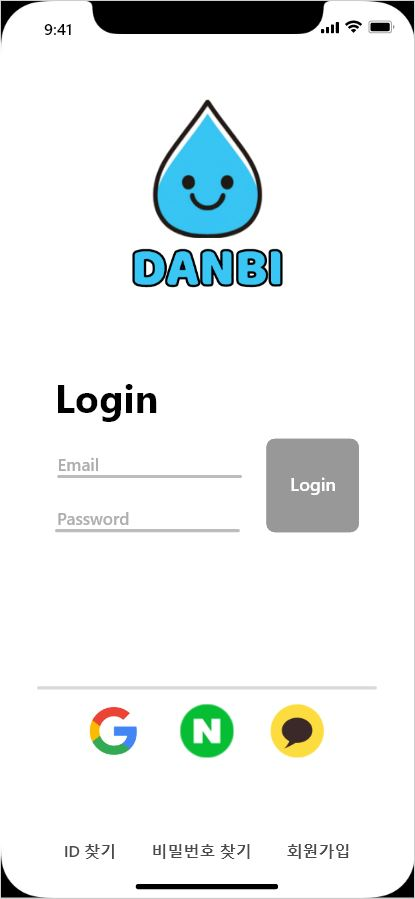
\includegraphics[width=3cm]{xd/login page.JPG}
\centering
\caption{}
\label{fig:login}
\end{figure}

[Fig. \ref{fig:login}] There are two text fields(Email, Password) in the 'Login page'. The user may log in by entering an Email and Password in the corresponding field. In the case of the Password field, the input value is changed as a dot. There is a login button on the right side of the text field. Under the two fields and login button, there are icons of 'Google', 'NAVER' and 'Kakao' that allow social login. If you press the login button after entering the correct information, application automatically provide the 'Main page'. At the bottom, there are find ID, find Password, and sign up buttons. If the user presses the sign up button, application automatically access the 'Sign Up page'. Account information can be recovered by touching finding ID and finding Password at the bottom.

\begin{enumerate}
\setlength{\parindent}{2ex}
\item Correct ID and Password

Account information is sent to the database when the user correctly enters the ID value(Email), Password and presses the login button. Database sends the data values stored about account to the server and processes them so that the application can show the data to the user. During this process, an ActivityIndicator(loading icon) is displayed. If the user log in successfully, the ActivityIndicator automatically disappears and the user accesses the 'Main page'.

\item Wrong ID or password

If the account information entered in the text field is not in the database, the error message "계정 정보가 없습니다. 아이디나 비밀번호를 확인해주세요." appears as pop up in the field. If the user touches to modify the field, the existing input value is automatically erased.

\item Account retrieval

Account information can be recovered by touching finding ID or finding Password at the bottom. If the user forgets the Email address registered with ID, she can recover it by entering the name and mobile phone number. The entered information is sent to the server, and database returns the account Email address that matches to information. The password is not a method of bringing up values stored in the database, but a method of registering a new Password. If the user forgets the Password, entering the ID and name will send the authentication code to the entered Email. Authenticating the code allows the user to set a new password. If the application have processed all the ID or Password changes requested by the user, it will automatically access the 'Login page' again.

\end{enumerate}

\item \textbf{Main Page}

\par \begin{figure}[h!]
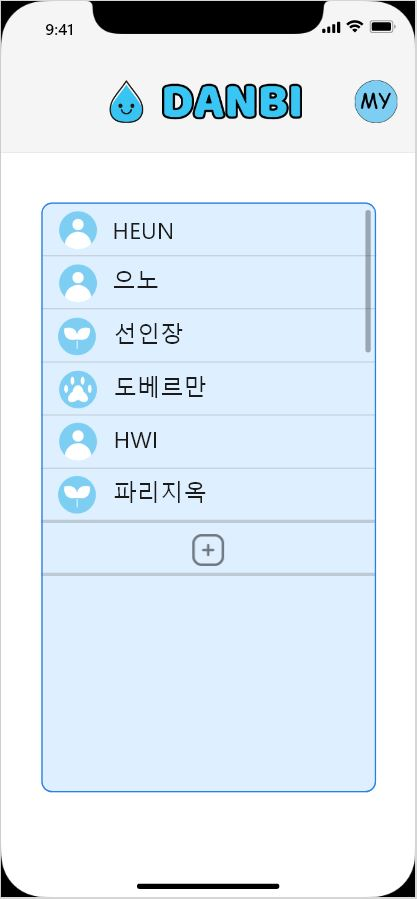
\includegraphics[width=3cm]{xd/main page.JPG}
\centering
\caption{}
\label{fig:main}
\end{figure}

[Fig. \ref{fig:main}] In 'Main page', the user can see a list of members registered in account. In DANBI, humans, pets, and plants can be registered as family members. The member's nickname is provided in the form of a list along with an icon representing each object, and when each nickname is clicked, the member's detailed screen page is accessed. There is a '+' button below the member list. When the button is clicked, application is automatically connected to the 'Member Registration page' where user can add members.

\item \textbf{My tab}

\par \begin{figure}[h!]
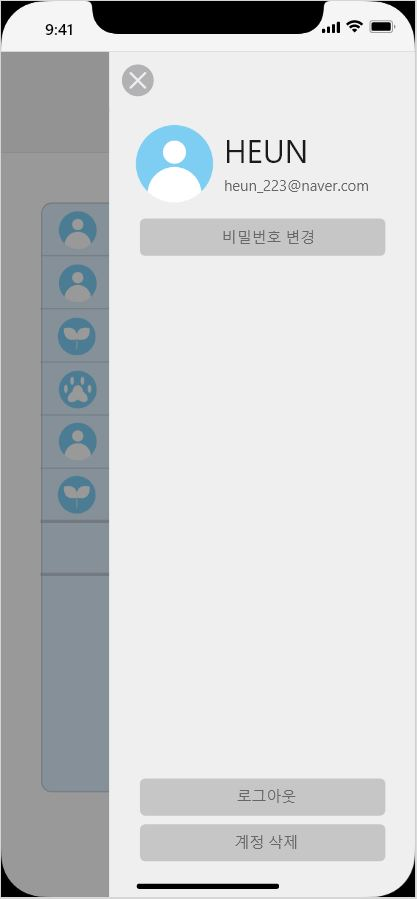
\includegraphics[width=3cm]{xd/my tab.JPG}
\centering
\caption{}
\label{fig:mytab}
\end{figure}

[Fig. \ref{fig:mytab}] In 'My tab', account information may be checked, edited, or deleted. Specifically, registered Email information may be checked and the Password may be changed through an authentication procedure. Logout is also possible, and when the user re-access to account after logging out, the user will be connected the "Login page" after the "Entry page" and have to log in to retrieve account information again. When deleting an account, all data of the user is deleted from the database.


\item \textbf{Member registration page}

\par \begin{figure}[h!]
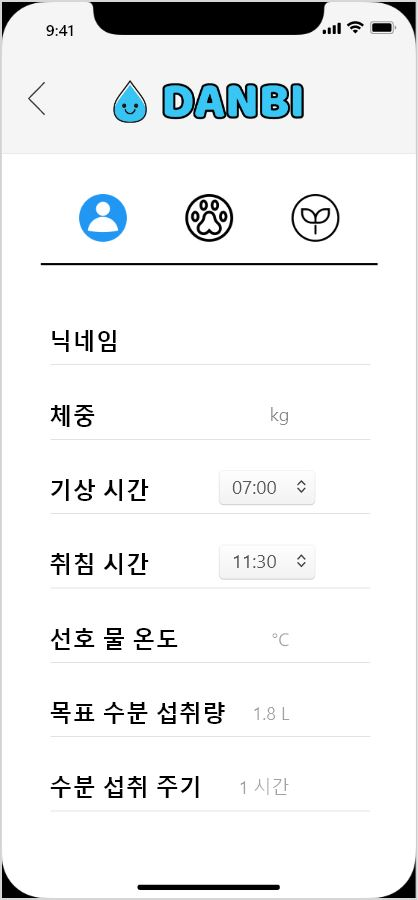
\includegraphics[width=3cm]{xd/member registration page.JPG}
\centering
\caption{}
\label{fig:registration}
\end{figure}

[Fig. \ref{fig:registration}] In the 'Member Registration page', information on new family members can be registered. The registered information is stored in the database and immediately added to the 'Main page', member list.
\begin{enumerate}
\setlength{\parindent}{2ex}
\item Human

Informations needed to add human member include nickname, weight, wake-up/bed time, preferred water temperature, water intake goal, and water intake cycle. The personal information of the input human is stored in the DANBI database. Based on the entered physiological information, the recommended daily water intake and the recommended cycle of water intake are provided. The recommended daily water intake is calculated as [ weight(kg) * 30(ml) ].\cite{waterIntake_Human} The recommended amount and recommended cycle of water intake can be changed by the user, and when it is confirmed, the amount of water intake is automatically calculated and provided to the user.
\item Pet

Informations needed to add pet member includes nickname, animal type(dog/cat), weight, wake-up/bed time, water supply goal, and water supply cycle. The input pet information is stored in the DANBI database. Based on the type and weight of the pet, the recommended water supply amount and recommended cycle of water supply are calculated and provided. \cite{waterIntake_Pet}

- Dog with a weight of 10kg or less : recommended amount of water supply is calculated as [ weight(kg) * 60(ml) ]

- Dog with a weight 11kg to 25 kg : recommended amount of water supply is calculated as [ weight(kg) * 50(ml) ]

- Dog with a weight 26kg or more : recommended amount of water supply is calculated as [ weight(kg) * 40(ml) ]

- Cat : recommended amount of water supply is calculated as [ weight(kg) * 45(ml) ]

The recommended amount and cycle of water supply can be changed according to the characteristics of the animals observed by the user, and when it confirmed, the amount of water supply is automatically calculated and provided to the user. The user can manage the water supply of pet accordingly.
\item Plant

Informations need to add plant member includes nickname, plant type, the. last water supply date, the water supply time, water supply amount at once, and water supply cycle. When adding plant members, the DANBI basically provides about 50 kinds of plants. If it does not exist in the provided plant, the user can add it. DANBI provides a recommended water supply cycle according to the input plant types. \cite{waterIntake_Plant} This can be changed by the user. In the case of the recommended amount of water supply, the user inputs it directly because it depends on the size of the plant.

\end{enumerate}
\item \textbf{Member Specification page}

\par \begin{figure}[h!]
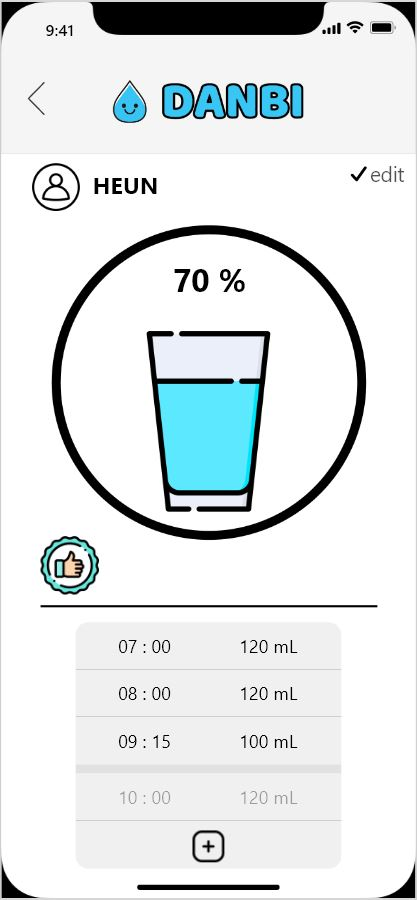
\includegraphics[width=3cm]{xd/member specification page.JPG}
\centering
\caption{}
\label{fig:specification}
\end{figure}

[Fig. \ref{fig:specification}] 'Member Specification page' provides data that visually analyzes of water intake information of a member. In addition, the input information may be edited. Specific informations provided include 'Today's achievement', 'Water Record', 'Award Stamp'. In addition, the page provide 'Edit Information' and 'Add New Water Record'.

\begin{enumerate}
\setlength{\parindent}{2ex}
\item Today's Achievement

It provides a visual representation of the member's daily water intake achievement in a graph. The graph is made based on information on the daily water intake and the daily intake goal stored in the database. User can visually check daily water intake and the remaining intake at a glance. Also the user can check a visual indication of how much water intake today is compared to daily water intake goal and how much more to reach the goal.
\item Water Record

Specific intake information of members can be checked. It provides the time and amount of water consumed during the day. Below that, it provides the next estimated time to have water intake. On a daily basis, the time of water intake stored in the database and the amount of water intake at that time are transmitted to the server, and the application visualizes and provides it for user.
\item Add New Water Record

The water intake information of the member may be manually input. In some cases, water intake information is not automatically recorded in the database, such as when drinking water other than pop up notification time or when a user pressed '미루기' to notification. In this case, the user manually inputs the time and amount of water intake to add data to the database.
\item Edit Information

In the case of humans, the information edit page contains information on Nickname, Weight, Wake-up/bed time, Preferred water temperature, Water intake goal, and Water intake cycle, and it is same with when adding members. The user can change all values. Among them, modifying the weight value provides a new recommended daily water intake regardless of the previously set value, which can also be changed by the user.

In the case of pets, the information edit page contains information on Nickname, Animal type(dog/cat), Weight, Wake-up/bed time, Water supply goal, Water supply cycle. All values except the type can be changed. Among them, when the weight value of the animal is edited, the recommended daily water intake and water supply cycle are recalculated and provided, which can be changed by the user.

In the case of plants, the information edit page contains information on Nickname, Plant type, The last water supply date, The water supply time, Water supply amount at once, Water supply cycle. All of these values can also be changed. Among them, when the type is edited, the recommended water supply cycle is provided again, which can be changed by the user.
\item Award Stamp

If a user presses the stamp button on the ‘Member specification page’, ‘Award stamp page’ appears and it have a calendar. When the water intake goal is completed, a stamp is stamped on that date. By pressing the triangle button on the left and right sides of the month, it shows the stamps of last and next months. If you press the X mark or select a screen outside the ‘Award stamp page’, the page is turned off.
\end{enumerate}
\item \textbf{Push / Pop Up Notification}

\par \begin{figure}[h!]
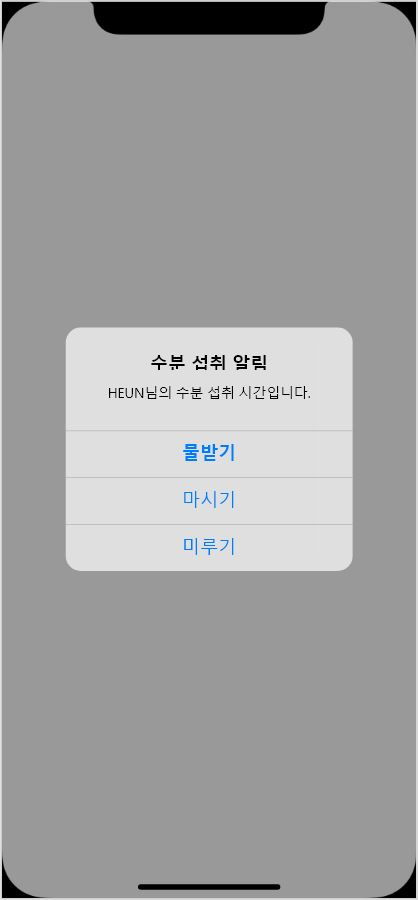
\includegraphics[width=3cm]{xd/notification.JPG}
\centering
\caption{}
\label{fig:notification}
\end{figure}

[Fig. \ref{fig:notification}] A notification appears on the mobile phone when the set water intake time comes. A pop-up notification appears when the user is using a mobile phone, and a push notification appears when not using it. It notifies the nickname and the amount of water intake of the member who need to drink water. Examples are as follows. - “OOO님의 수분 섭취 시간입니다. OOOml 섭취하세요.”

There are three buttons that the user can select in the notification. There are ‘물받기’, ‘마시기’, ‘미루기’. The application reacts differently depending on which button the user presses.
\begin{enumerate}
\setlength{\parindent}{2ex}
\item When selecting ‘물받기’, the LG PuriCare water purifier connected to the application offers water according to the amount of water intake at once and water temperature set by the user. It also delivers the amount of water intake and the time when the button is pressed to the server, stores it in the database, and updates the application.

\item When selecting '마시기', the amount of water intake and the time when the button is pressed are delivered to the server, stored in the database, and the application is updated.

\item When '미루기' is selected, the application immediately removes the notification and does not update anything.
\end{enumerate}

The notification disappears immediately when the user presses the button on the option. However, after the notification appears for 5 seconds, if the user does not press any button within that time, the application automatically selects ‘미루기’.
\end{itemize}

\subsection{NUGU speaker}
\begin{itemize}
\setlength{\parindent}{2ex}
\item \textbf{Notification}

In the same way as the notification of the application, when the water intake time set by the user comes, NUGU speaker notifies the user by voice as follows. - “OOO님의 수분 섭취 시간입니다.”

The reactions that users can make to the notification are '물받기', '마시기', '미루기', which are the same as the reactions in the application. If you want to choose ‘물받기’, you can answer "물 받아줘" to NUGU speakers. If you want to choose ‘마시기’, you can answer "물 마실게" to NUGU speakers. If you want to choose ‘미루기’, you can answer "나중에 마실게" to NUGU speakers. When the user inputs one of the three reactions by voice, the system's response is also the same as in the application. If there is no response from the user for 10 seconds after the notification of the NUGU speaker, '미루기' is automatically selected and DANBI is terminated.

\item \textbf{Communication}

To execute DANBI, the user should say, "단비 켜줘." As the application in NUGU speaker runs, NUGU speaker says, "단비를 실행합니다."

The user can ask three types of questions. There are questions that can check today's water intake, the last time of water intake, and the next time of water intake.

\begin{enumerate}
\setlength{\parindent}{2ex}

\item To check how much water the member intakes today, the user can ask NUGU speaker, “OOO 오늘 물 얼마나 마셨어?” with the nickname of the member that the user wants to check. Then based on the daily water intake stored in the database, NUGU speaker says, “OOO님은 오늘 OOOml(혹은 OL) 마셨습니다. 목표 섭취량까지 OOOml(혹은 O.OL) 남았네요.” If the amount of water is less than 1L, it is guided in ml to deliver the exact value to the user, but if it is more than 1 liter, it is guided in L units to help understand faster. In addition, to prevent the message from getting too long in unit L, it guides upto only one decimal place.

\item The user can ask NUGU speaker when the last water intake time is. If the member you want to check is a human, you can say with the member's nickname, “OOO 언제 물 마셨어?” If a member is a pet or plant, add the member's nickname and say, “OOO 언제 물 줬어?” The NUGU speaker takes the last water intake date and time stored in the database through the server and guides it as follows. In the case of humans and pets, they drink water every day, so along with the time excluding the date, they say, “OOO님의 마지막 수분 섭취 시간은 OO시 (OO분) 입니다.” It guides the time, and if it is at prompt, the notification is concise by omitting how many minutes it is. In addition, if there is no record of water intake yet within a day, it says “OOO님은 아직 오늘의 수분 섭취가 없습니다.” In the case of plants, the interval between water intake is by date, so they say, “OOO님의 마지막 수분 섭취 날짜는 O월 O일입니다.”

\item The user can also ask NUGU speaker when the next water intake time is. If the member you want to check is a person, you can say with the member's nickname, “OOO 언제 물 마셔야 돼?” If a member is an animal or plant, you can add the member's nickname and say, “OOO 언제 물 줘야 돼?" NUGU speaker takes the date and time of water intake from the database through the server and guides it as follows. In the case of humans and animals, they drink water every day, so along with the time excluding the date, they say, “OOO님의 다음 수분 섭취 시간은 OO시 (OO분)입니다.” In addition, if the guidance time is at prompt, minutes are omitted. In the case of plants, the water supply cycle is by date, so along with the date, they say, “OOO님의 다음 수분 섭취 날짜는 O월 O일입니다.”
\end{enumerate}

The notification disappears immediately when the user presses the button on the option. However, after the notification appears for 5 seconds, if the user does not press any button within that time, the application automatically selects ‘미루기’.

\end{itemize}

\subsection{LG PuriCare}
\setlength{\parindent}{2ex}

When a user selects "물받기" in response to an application notification or NUGU speaker's voice notification, the server sends a query to the LG PuriCare water purifier about the temperature and amount of water set differently for each member. The LG PuriCare water purifier receives the query and automatically offers water according to the set value.


\begin{thebibliography}{00}
\bibitem{waterIntake_Human} 
\url{http://kwater.or.kr/web/download/info/WRqna.pdf}

\bibitem{waterIntake_Pet}
\url{https://www.notepet.co.kr/news/article/article_view/?idx=17654}

\bibitem{waterIntake_Plant}
\url{https://fuleaf.com/#filter}


\end{thebibliography}
\end{document}
